\chapter{Versuch 1}
\label{chap:VERSUCH_1}

\section{Fragestellung, Messprinzip, Aufbau, Messmittel}
\label{chap:VERSUCH_1_FRAGESTELLUNG}

Bei Versuch 1 ging es um die Messung von Abständen mittels eines Entfernungssensors. 

\subsection*{Fragestellung}

	Sinn: Abstände mittels Sensor messen um dann Fehler zu ermitteln
\subsection*{Messprinzip}
	Der Sensor sendet mit einer LED ein rotes Licht aus, das vom Objekt reflektiert und dann von einen optischen Positionssensor (OPS) wider erfasst wird. Die Leitfähigkeit des OPS ist von der Einfallposition des Lichts abhängig, so ergeben unterschiedliche Einfallspositionen unterschiedliche Spannungen, aus denen sich dann der Einfallswinkel berechnen lässt. Aus diesen kann man dann über das Triangulationsprinzip die Entfernung ermittelt.
	
	(Quellverweis einfüge: ist von der Versuchsanleitung)
	\begin{center}
	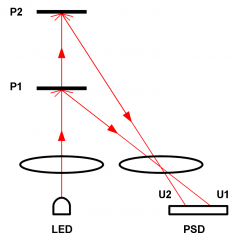
\includegraphics[scale=1]{media/triangulationGraphik.png}
	\label{Triangulation}
	\end{center}
	
	
\subsection*{Aufbau}

	\includegraphics[scale=0.15]{media/aufbau.png}
	\label{Versuchsaufbau}

	
\subsection*{Messmittel}
\ref{Versuchsaufbau}
	Zur Messung wurden folgende Messmittel benutzt:
	\begin{itemize}
		\item Sensor(Abstandmessungssensor)
		\item Osziloskop		
		\item Metermaß
		\item Brett (als Objekt dessen Abstand gemessen wird)
	\end{itemize}

\section{Messwerte}
\label{chap:VERSUCH_1_MESSWERTE}
	\begin{tabular}{|c|c|}
	\hline 
	Abstand in cm & Spannung in V \\ 
	\hline 
	10  & 1,363 \\ 
	\hline 
	13 & 1,212 \\ 
	\hline 
	16 & 1,078 \\ 
	\hline 
	19 & 0,973 \\ 
	\hline 
	22 & 0,897 \\ 
	\hline 
	25 & 0,822 \\ 
	\hline 
	28 & 0,765 \\ 
	\hline 
	31 & 0,699 \\ 
	\hline 
	34 & 0,656 \\ 
	\hline 
	37 & 0,637 \\ 
	\hline 
	40 & 0,599 \\ 
	\hline 
	43 & 0,560 \\ 
	\hline 
	46 & 0,541 \\ 
	\hline 
	49 & 0,523 \\ 
	\hline 
	52 & 0,523 \\ 
	\hline 
	55 & 0,504 \\ 
	\hline 
	58 & 0,485 \\ 
	\hline 
	61 & 0,485 \\ 
	\hline 
	64 & 0,485 \\ 
	\hline 
	67 & 0,485 \\ 
	\hline 
	70 & 0,466 \\ 
	\hline 
	\end{tabular} 
	\label{WerteHand}

	
	

\section{Auswertung}
\label{chap:VERSUCH_1_AUSWERTUNG}
	
	
\section{Interpretation}
\label{chap:VERSUCH_1_INTERPRETATION}
